\chapter{Methods}
\label{Methods}
\thispagestyle{empty}

In this chapter we will give an outline of the experimental choices we made to fulfill the MDP elements described in Chapter \ref{Problem_Statement}.

At first, we will discuss about the state and the reward function.
Then, we will describe the algorithm which is the core of this thesis work:
In the first part we will describe the parametric rule-based policy $\psi_{\boldsymbol \omega}$ that we adopted to follow the reference trajectory and that we will call controller from now on. In the second part we will illustrate the parametric policy aimed at improving the performance which we implemented as an RL agent.
Finally, we will discuss other approaches that try to learn an imitating and improving policy directly.

\section{Observation}
\label{sec:obs}

TORCS, at each time-step $t$, sends many data representing telemetry information. This is what in Fig.\ref{fig:diagram3} is referred as $X_t$.
Not all the data coming from the simulator are used as the state representation.
The state is defined as a vector of features that represent different sensors readings which include position, velocity, acceleration, angle of the car with respect to the track axis and 19 range finder sensors, where each sensor represent the distance between the track edge and the car.
So, these data, after an initial filtration, are split in two arrays: one is fed to the controller, one to the improving agent.

The telemetry data sent from TORCS and used to construct the two observation vectors are:

\begin{itemize}
\item $x$ is the $x$ component of the position with respect to the TORCS reference system.
\item $y$ is the $y$ component of the position with respect to the TORCS reference system.
\item $yaw$ is the angle with respect to the absolute coordinate system, i.e., $0$ for the point $(1,0)$, $\frac{\pi}{2}$ for the point $(0,1)$ and $-\frac{\pi}{2}$ for the point $(0,-1)$.
\item $speed_x$ is the speed of the car along the longitudinal axis of the car.
\item $speed_y$ is the speed of the car along the transverse axis of the car.
\item $acceleration_x$ is the acceleration of the car along the longitudinal axis of the car.
\item $acceleration_y$ is the acceleration of the car along the transverse axis of the car.
\item $angle$ is the angle between the car direction and the track axis.
\item $trackPos$ is the distance between the car and the track axis.
\item $trackSensors$ is a vector of 19 range finders: each sensors returns the distance between the track edge and the car within a range of 200 meters. The sensors sample the space in front of the car every 10 degrees, spanning clockwise from -90 degrees up to
+90 degrees with respect to the car axis.
\end{itemize}

In the sections \ref{RB_state} and \ref{ppostate}, we go into the details about the input states $X^\psi$ and $X^\pi$ of the controller and the improving agent respectively.


\section{Reward Functions}
\label{sec:reward_function}
\begin{figure}
    \centering
 	  \captionsetup{width=10cm}
      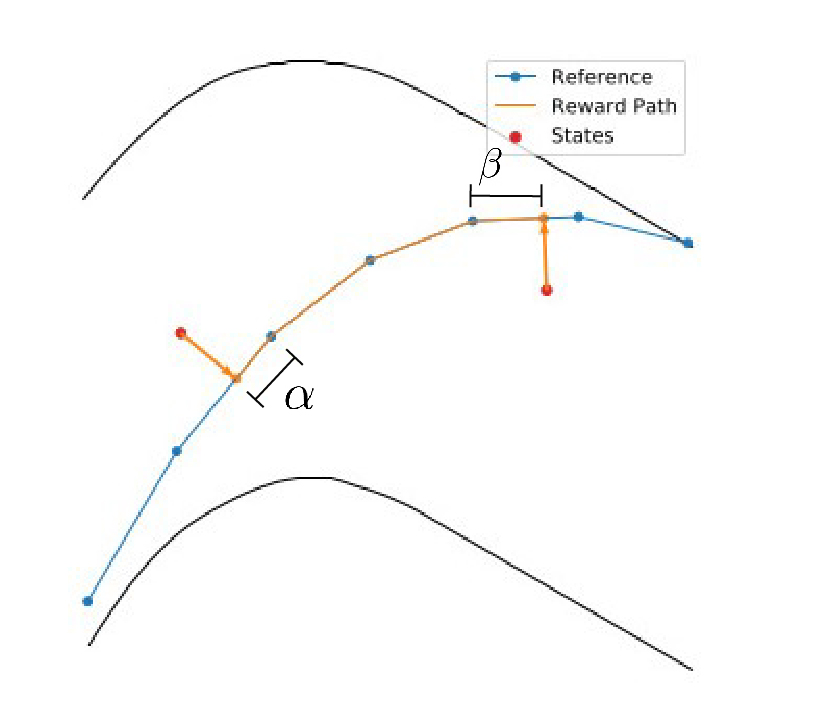
\includegraphics[width=10cm]{./img/reward2}
     \caption{Example of arc between two states projected on the reference trajectory. In this situation, for sake of simplifying the picture, the sampling frequency of the reference trajectory is twice the sampling frequency of the pilot}
   \label{fig:reward}
  \end{figure}
The reward function $r(S_t,A_t)$ defines the agent's performances with respect to the expert in the nearby of its position. Consequently, if the agent performs better than the reference trajectory in the nearby of a position $(x,y)$, it will receive a positive reward. Contrarily, it will receive a negative reward.

The reward is defined as the relationship between the two consecutive states and the reference trajectory. To reduce the error due to the discretization of the trajectories, the states are projected on the reference trajectory and to compute the reward we consider the arc between the two projected points. Figure \ref{fig:reward} illustrates this idea showing two consecutive states, their projection on the reference trajectory and the arc considered for the computation of the reward. Then we defined three reward functions as difference respectively of the time, distance and average speed between pilot and reference trajectory on the arc.

\textbf{Time reward function}: The time reward function measures the time that the pilot has gained/lost with respect to the reference trajectory between two consecutive samples. This function is defined as:
\begin{equation} r_{\text{time}} = t^{\text{pilot}}_i - (t^{\text{ref}}_{p_{i+1}} - t^{\text{ref}}_{p_i} )\end{equation}
where \(t^{\text{pilot}}_i\) is the elapsed time between the $i^{th}$ and the $(i+1)^{th}$ states and $p_i$ is the projection on the reference trajectory.
It is important to point out that $t^{\text{pilot}}_i$ is constant, $t^{\text{pilot}}_i=0.1 \text{s}$, because it depends on the pilot sampling frequency. $t^{ref}_{p_i}$ is the time of the projection on the reference trajectory, and it depends on the position of the pilot.
In Fig. \ref{fig:reward}, for example, we can compute
\begin{equation}(t^{\text{ref}}_{p_{i+1}} - t^{\text{ref}}_{p_i} ) = 2\Delta t_{ref} + (\alpha + \beta)\Delta t_{ref}
\label{eq:t_ref}\end{equation}
where $\Delta t_{ref}=1/f_s^{ref}$ is the time elapsed between two consecutive states of the reference trajectory and $\alpha$ and $\beta$ are the proportions of the segments upon which the projections lay.
To summarise, $(t^{\text{ref}}_{p_{i+1}} - t^{\text{ref}}_{p_i} )$ is the time that the reference trajectory takes to travel from the projection $p_i$ to $p_{t+1}$. Thus, the difference $r_{time}$ corresponds to the time difference between the performance of the pilot and the one of the reference trajectory on that specific arc.


\textbf{Space reward function}: The space reward function measures the difference between the distance driven by the pilot and the reference trajectory. This function is defined as:
\begin{equation}
\label{eq:r_space}
 r_{\text{space}} = d^{\text{pilot}}_i - (d^{\text{ref}}_{p_{i+1}} - d^{\text{ref}}_{p_i} )\end{equation}
where \(d^{\text{pilot}}_i\) is distance between the $i^{th}$ and the $(i+1)^{th}$ states and $d^{ref}_{p_i}$ is the distance traveled by the reference trajectory between the projections.
The same reasoning made for the time reward function, regarding the meaning of the formula, can be done for the space reward function, by substituting the time $t$ with the distance $d$ in the equation \ref{eq:t_ref}.

\textbf{Speed reward function}: The speed reward function measures the average speed difference between pilot and reference trajectory on the considered arc. This function is defined as:
\begin{equation}r_{\text{speed}} = \frac{d^{\text{pilot}}_i}{t^{\text{pilot}}_i} - \frac{d^{\text{pilot}}_i}{t^{\text{ref}}_{p_{i+1}} - t^{\text{ref}}_{p_i} }\end{equation}
where \(t^{\text{pilot}}_i\) and  \(d^{\text{pilot}}_i\) are respectively the elapsed time and distance between the $i^{th}$ and the $(i+1)^{th}$ states and $p_i$ is the projection on the reference trajectory. ${d^{\text{pilot}}_i}/{t^{\text{pilot}}_i}$ is the average speed of the pilot that goes from the state at time $i$ to the state at time $i+1$. ${d^{\text{pilot}}_i}/({t^{\text{ref}}_{p_{i+1}} - t^{\text{ref}}_{p_i} })$, instead, is the reference trajectory average speed along that distance.


\subsection{Episode stopping criteria}
An episode ends when the agent comes in a terminal state: if the car reaches the endline, the episode is considered successful and the reward is 0.
In the other cases listed below, the episode is considered a failure, and a negative reward is given as penalty.
\begin{itemize}
    \item If the car goes out of the boundary of the track with half of its width, the episode is early stopped. This is explained by two reasons: by going out of track, the car is slowed down by the rough terrain, which obviously makes it impossible to obtain the best time. Secondly, it grants avoiding cutting the curves without following the track, which is forbidden.
    \item If the car hits a wall, the episode is stopped. In some occasions, this coincide with the previous case, because in these situations the boundary of the track is a wall itself.
    \item If the car's speed is lower than $5$kmh, the episode is stopped. Since at the beginning of each episode the car is driving far faster than this speed, this event would mean that the car is going too slow.
    \item If the car is driving backwards, obviously it's impossible to obtain the best result and the episode is stopped. This event may occur when the car incurs in a spin.
\end{itemize}




\section{Proximal Policy Optimization upon Rule-Based Parametric Policy}
A solution that we implemented to the aim of finding the best lap-time is composed of a two-phase optimization problem.
The former can be viewed as an imitation learning problem, where goal is to follow as much as possible the reference trajectory.
To this end, we implemented a controller, i.e., a rule-based parametric policy $\psi_{\boldsymbol \omega}$, with $\boldsymbol \omega$ parameter vector, which seeks to minimize the difference between the agent trajectory and the human demonstration. 
In order to optimize the parameters of this policy, we chose to adopt a Policy Gradient algorithm, in particular POIS (see Section\ref{sec_POIS}).
In the next section, we will discuss the details about the implementation of this solution.
The second phase begins after that the optimal policy $\psi_{\boldsymbol \omega^*}$ is found. To this end, we implemented an RL agent whose aim is to learn a parametrized policy $\pi_{\boldsymbol \theta}$ that finds the best lap-time. In order to optimize this policy, we adopted the RL algorithm PPO (see Section \ref{ppo}).

\subsection{Rule-based Parametric Policy}
In this section, we discuss the choices we made to implement and optimize the policy $\psi_{\boldsymbol \omega}$ aimed at following the reference trajectory. In the first part we give a detailed formulation of the policy structure and parameters, then we explain how we adopt P-POIS algorithm, described in Section \ref{sec_POIS}, to optimize these parameters.

\subsubsection{State}
\label{RB_state}
The state consists in an input $X^{\psi}_t$ composed by three variables $x$, $y$, $yaw$, $speed_x$, $speed_y$ and $trackPos$. The features $x$, $y$ are necessary only to find the nearest reference trajectory point. From the other inputs, the delta feature $\rho$, $\Delta v$ and $\Delta \theta$, relative to the reference trajectory, are computed. Details of their computation will be given in Section \ref{seq:rule_b_algo}.
From these delta features, the controller computes the action $A^{\psi_{\boldsymbol \omega^*}}_t$ that is meant to bring the car as close as possible to the reference trajectory.

\subsubsection{Algorithm}
\label{seq:rule_b_algo}
The policy $\psi_{\boldsymbol \omega}$ acts upon three actions: \textit{throttle}, \textit{brake} and \textit{steer}.
Each action uses a different set of features. Their objective is to minimize these features with respect to the reference trajectory.
\newline  \textbf{Brake} The brake is defined as:
\begin{equation}B(t)=\beta(v^{\text{pilot}}_x(t)-v^{\text{ref}}_x(t)),\end{equation} where $B(t)$ is clipped between 0 and 1, $v^{\text{pilot}}_x(t)$ is the longitudinal component of the speed of the pilot at time $t$ and $v^{\text{ref}}_x(t)$ is the longitudinal component of the speed of the orthogonal projection on the reference trajectory at time $t$.
The brake is actuated proportionally to the difference of the speed of the pilot and the speed of the reference. It is clipped between 0 and 1 because they are the maximum and the minimum limits allowed by TORCS.
\newline  \textbf{Throttle} The throttle is defined as:

\begin{equation}
    \Tilde{T}=max\{ \alpha_1(v_x^{\text{ref}}(t)-v_x^{\text{pilot}}(t)), 1 \}
\end{equation}

\begin{equation}
  T(t) =
    \begin{cases}
      0 &
      \text{$\Tilde{T}-\alpha_2 v_y^{pilot} \leq 0$} \\
      
      \Tilde{T}-\alpha_2 v_y^{pilot} &
      \text{$v_y^{pilot} \geq \alpha_3 \wedge \Tilde{T}-\alpha_2 v_y^{pilot}<0$}\\
      
      
      \Tilde{T} &
      \text{$v_y^{pilot} < \alpha_3 \wedge \Tilde{T}-\alpha_2 v_y^{pilot}<0$}\\
    \end{cases}       
\end{equation}

where $v^{\text{pilot}}_y(t)$ is the lateral component of the speed of the pilot at time $t$.
The throttle is actuated if the car is traveling at a lower speed than the reference trajectory. Furthermore, a discount to the throttle is applied if the lateral speed $v_y^{pilot}$ is above a threshold parameter $alpha_3$. This is to avoid a too harsh acceleration during a turn, that can result in sliding of the car.
\newline  \textbf{Steer} The steer is defined as:
\begin{equation}
\begin{split}
S(t) & = 
   \frac{1}{4} \big(S(t-1)+
    [S(t-1)+\Delta f(\rho;\gamma_1)]+\\
    &[S(t-1)+\Delta f(\theta;\gamma_2)]+
    [S(t-1)+\Delta f(A;\gamma_3)] \big) \\
 & = S(t-1)+\frac{1}{4} \Delta f(\rho;\gamma_1) + \frac{1}{4} \Delta f(\theta;\gamma_2)+ \frac{1}{4} \Delta f(A;\gamma_3)
\end{split}
\end{equation}


where:
\begin{itemize}
    \item $f(x;\gamma)$ is the transformation function defined as:
\begin{equation}f(x;\gamma)=tanh(\gamma x),\end{equation}
This transformation is applied to maintain the steer between the range [-1;1].
\item $\Delta f(x;\gamma)$ is the delta of the transformation function between the time step $t$ and the time step $t-1$:
\begin{equation}\Delta f(x;\gamma)=f(x(t);\gamma)-f(x(t-1);\gamma),\end{equation}
\item $\rho$ is the distance between the car trajectory and the reference trajectory:
\begin{equation}\rho=\frac{trackPos_{ref}-trackPos_{pilot}}{2},\end{equation}
\item $\theta$ is the delta car orientation:
\begin{equation}
    \theta = \frac{yaw_{ref}-yaw_{pilot}}{2\pi}
\end{equation}
\item A is the track curvature:
\begin{equation}A=\frac{yaw_{ref+k}-yaw_{ref}}{2\pi},\end{equation}
where $k$ is the number of steps forward.
\end{itemize}

To outline the steer, it is the average of four components: the steer at the previous time step; the steer at the previous time step plus the increment proportional to the distance between the car and the reference trajectory; the steer at the previous time step plus the increment proportional to the orientation of the car with respect to the reference trajectory; the steer at the previous time step plus the increment proportional to the track curvature.
The meaning of the steer is that each of the four components estimates the steer necessary to minimize its own delta feature. Then, the results are averaged. The meaning of every component is the increment upon the the steer at the previous time step.
This means that, for example, if a delta components are equal to zero, the steer of the previous time step is applied. The increment is represented by $\Delta f$ which is the difference between the target steer at time $t$ and the one at time $t-1.$

To give an example: if at time $t-1$ a given delta component required a steer of $0.5$ and at time $t$ the same component requires $0.2$, then delta will be equal to $-0.3.$






\subsubsection{Policy Optimization}
In order to find the best controller, we need to optimize the parameter vector 
\[
\boldsymbol \omega= 
\begin{bmatrix}
\alpha_1  & \alpha_2 & \alpha_3 & \beta & \gamma_1 & \gamma_2 & \gamma_3
\end{bmatrix}'.
\]
Indeed, these are the parameters that influence the behaviour of the controller. By finding the optimal $\boldsymbol \omega^*$, we obtain the controller that best approximates the reference trajectory, as good as possible.
We chose to adopt P-POIS as optimizer, as it adopts a parameter-based approach, allowing the exploration over the parameter space.
Moreover, it performs an offline trajectory optimization at each iteration. At each iteration the algorithm fixes the hyperpolicy and generates a set of trajectories sampling the parameters of the policy. The sets of parameters and their corresponding reward are the input for the offline optimization, which result gives a new hyperpolicy for the next iteration.

In order to approximate the reference trajectory, a Gaussian hyperpolicy $\nu_{\boldsymbol \rho}$ with diagonal covariance matrix is used, $\mathcal{N}(\boldsymbol \omega,diag(\boldsymbol \sigma^2))$, belonging to a hyperpolicy space \(\mathcal{N}_{\mathcal{P}} = \{\nu_{\boldsymbol \rho}:\boldsymbol \rho \in \mathcal{P} \subseteq \mathbb{R}^r\}\). The hyperpolicy is used to sample the policy parameters $\boldsymbol \omega$ at the beginning of each episode.
Our goal is to determine the hyperparameters \(\boldsymbol \rho^*\) so as to maximize \begin{equation} J_D( \boldsymbol \rho) = \int_{\Theta} \int_{\mathcal{T}} \nu_{\boldsymbol \rho}( \theta)p(\tau| \boldsymbol \omega)R(\tau)d\tau d \boldsymbol \omega,  \label{eq:jdro} \end{equation} where $p(\tau|\boldsymbol \theta)$ is the trajectory density function. 

To this end, P-POIS adopts a surrogate loss function
\begin{equation}\mathcal{L}_\lambda(\boldsymbol \rho'/\boldsymbol \rho)=\frac{1}{N} \sum^N_{i=1}\epsilon{\boldsymbol \rho'/ \boldsymbol\rho}(\boldsymbol \omega)R(\tau_i)-\lambda\sqrt{\frac{d_2(\nu_{\boldsymbol \rho'}\|\nu_{\boldsymbol \rho)}}{N}},\end{equation} where 
\(\epsilon_{\boldsymbol \rho'/\boldsymbol \rho}(\boldsymbol \omega)=\frac{\nu_{\boldsymbol\rho'}(\boldsymbol\omega)}{\nu_{\boldsymbol \rho}(\boldsymbol\omega)}.\)
Each trajectory $\tau_i$ is obtained by running an episode with action policy $\pi_{\boldsymbol \omega_i}$, and the corresponding policy parameters $\boldsymbol \omega_i$ are sampled independently from hyperpolicy $\nu_{\boldsymbol \rho}$ at the beginning of each episode. The hyperpolicy parameters are then updated offline as: \begin{equation}\boldsymbol \rho^j_{k+1}=\boldsymbol \rho^j_k+\alpha_k\mathcal{G}(\boldsymbol \rho_k^j)^{-1}\nabla_{\boldsymbol \rho_k^j}\mathcal{L}(\boldsymbol\rho^j_k/\boldsymbol \rho^j_0),\end{equation} where $\alpha_k > 0$ is the step size and $\mathcal{G}(\boldsymbol \rho^j_k)$ is the Fisher Information Matrix, which is a positive semi-definite matrix used to estimate the gradient with natural gradient \cite{fisher}.


\subsection{Proximal Policy Optimization}
In this section, we describe the parametric policy $\pi_{\boldsymbol \theta}$ which acts upon $\psi_{\omega^*}$. In particular, we implemented a Proximal Policy Optimization (PPO) algorithm aimed at improving the lap-time. 
Whe chose to adopt PPO being it relatively fast at learning and for its generalization capability.

\subsubsection{State}
\label{ppostate}
The state $X^{\pi}_t$ seen by the  agent is composed of $x$, $y$, $yaw$, $speed_x$, $speed_y$ , $acceleration_x$, $acceleration_y$, $angle$, $trackSensors.$ These vector of features $\Phi$ and the action $A^{\psi_{\boldsymbol \omega^*}}_t$, computed by the controller, are then combined to compose the input state $S$ of the improving agent. It is important to note that this input state does not refer to the reference trajectory, because this information is already in the action computed by the controller.



\subsubsection{Algorithm}

PPO alternates between sampling data through interaction with the environment, and optimizing a “surrogate” objective function using stochastic gradient ascent. While standard policy gradient methods perform one gradient update per data sample, PPO adopts multiple epochs of minibatch updates. 
The standard function adopted by PPO is is formulated as:
\begin{equation}
    \mathcal{L}^{PPO} = \mathcal{L}_t^{CLIP+VF+S}(\boldsymbol \theta) = \mathbb{E}_t\left[\mathcal{L}^{CLIP}_t(\boldsymbol \theta) -c_1 \mathcal{L}_t^{VF}(\boldsymbol \theta) + c_2[\pi_{\boldsymbol \theta}](s_t)\right],
\end{equation}
where $c_1$,$c_2$ are coefficients, $S$ denotes an entropy bonus, $L_t^{VF}$ is a squared-error loss $\left(V_{\boldsymbol \theta}(s_t)-V_t^{targ}\right)^2$, and $\mathcal{L}^{CLIP}_t$ is the loss function of Clipped Surrogate Objective:
\begin{equation}
    \mathcal{L}^{CLIP}(\boldsymbol \theta) = \mathbb{E}\left[\text{min}(r_t(\boldsymbol \theta) \hat{A_t},clip(r_t(\boldsymbol \theta),1-\epsilon,1+\epsilon)\hat{A_t}\right],
\end{equation}
where $r_t(\boldsymbol \theta) = \frac{\pi_{\boldsymbol \theta}(a|s)}{\pi_{\boldsymbol \theta_{old}(a|s)}}$, is the probability ratio so $r(\boldsymbol \theta)=1,$ $\epsilon$ is a hyperparameter, and the clipping term modifies the surrogate objective by clipping the probability ratio, which removes the inventive for moving $r_t$ outside of the interval $[1-\epsilon,1+\epsilon]$.

The goal of this policy is to improvement the action of the controller. Since we assume the controller to behave reasonably well, the goal is to obtain just a little improvement. Thus, we chose not to perform a vast exploration. This translates into a small action standard deviation. Hence, we chose not to include the entropy bonus factor in the loss function:
\begin{equation}
    \mathcal{L} = \mathcal{L}_t^{CLIP+VF}(\boldsymbol \theta) = \mathbb{E}_t\left[\mathcal{L}^{CLIP}_t(\boldsymbol \theta) -c_1 \mathcal{L}_t^{VF}(\boldsymbol \theta)\right].
\end{equation}

By definition, PPO adopts a stochastic policy, but it is our desire to make the driver deterministic.
Hence, once the best policy is found, for each state, PPO computes an action probability distribution from which to sample an action to perform. We, instead, select the mean value of such probability distribution.

\section{Direct Policies}
Another approach we adopted to tackle the problem of this thesis, is not to structure a two-step policy but to try and learn to follow and improve the reference trajectory all at once, with a monolith approach.
\subsection{FQI}
Fitted Q iteration is a batch mode reinforcement learning algorithm which yields an approximation of the Q-function corresponding to an infinite horizon optimal control problem with discounted rewards, by iteratively extending the optimization horizon \cite{fqi}.
We chose to apply this algorithm to our problem since it adopts a batch approach, which is convenient for us having a dataset of state-action values.

The algorithm consists in an iterative supervised learning problem, whose Q-function we chose to implement with an extra-trees \cite{extratrees}.

\subsection{DDPG}
ddpg per usare il replay dell'actor

